\question{Коэффициент поглощения и усиления активной среды. Сечение
поглощения}

\subquestion{Коэффициент поглощения активной среды. Сечение поглощения}
\begin{figure}[h!]
    \center
    \vspace{-3em}
    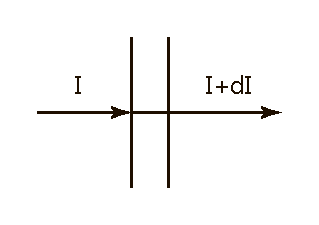
\includegraphics[width=.4\textwidth]{07_01}
    \vspace{-3em}
\end{figure}
При прохождении излучения через элементарный слой вещества \( dx \) его
интенсивность изменится на \( dI = -\alpha I\,dx \).

Поглощение света в прозрачных средах носит резонансный характер. Энергия
поглощенных фотонов пропорциональна количеству резонансных переходов
\[
    dI = W( n_2 - n_1 ) h\nu dx \quad \left(
      \frac{1}{\text{с}} \cdot \frac{1}{\text{м}^3} \cdot \text{Дж} \cdot
      \text{с} \cdot \frac{1}{\text{с}} \cdot \text{м} =
      \frac{\text{Вт}}{\text{м}^2} \right).
\]
Коэффициент поглощения \( \alpha \) можно выразить через сечение поглощения
\( \sigma \):
\[
    \alpha = \sigma( n_1 - n_2 ).
\]

\emph{Сечение поглощения (эффективное сечение)} -- площадь поперечного сечения
такой области пространства вокруг частицы, при пересечении которой фотон со
100\% вероятностью взаимодействует с ней. Обычно,
\( \sigma = 10^{-14} \ldots 10^{-26} \text{ м}^2 \).

\subquestion{Зависимость коэффициента поглощения от насыщающего излучения}
\begin{figure}[h]
    \center
    \vspace{-3em}
    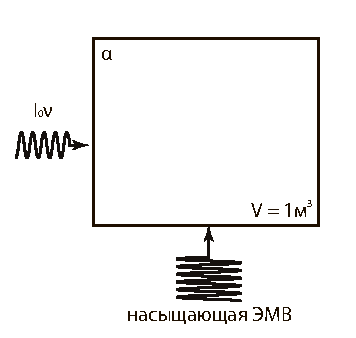
\includegraphics[width=.4\textwidth]{07_02}
    \vspace{-1.5em}
\end{figure}

Рассмотрим активную среду с инверсной населенностью
\( \D n = -n / (1 + 2W\tau) \).

Изменение интенсивности света, проходящего через среду, равно
\[
  dI = W( n_2 - n_1 ) h\nu\,dx. \quad \text{С другой стороны,} \quad
    dI = -\alpha I\,dx = -\sigma( n_1 - n_2 )I\,dx.
\]

Тогда вероятность индуцированных переходов:
\[
    W = \frac{dI}{(n_2 - n_1)h\nu dx} =
        \frac{-\alpha I dx}{(n_2 - n_1)h\nu dx} =
        \frac{\sigma(n_2 - n_1)I}{(n_2 - n_1)h\nu} = \frac{\sigma I}{h\nu}.
\]

Введём величину:
\(
  I_s(\sigma, \tau, \nu) = \cfrac{h\nu}{2\sigma\tau}, \left(
    \dfrac{\text{Вт}}{\text{м}^2}\right)
\). Тогда
\[
    \frac{\D n}{n} = -\frac{1}{1 + 2\sigma I\tau / (h\nu)} =
        \frac{-1}{1 + I / I_s},
\]
где \( I_s \) -- интенсивность насыщения перехода, зависящая только от параметров
среды.

В случае резонансного поглощения \( \nu = \nu_0 \) получаем зависимость:
\[
  \D n = \frac{-n}{1 + I / I_s}, \quad
    n_1 - n_2 = \frac{n}{1 + I / I_s}, \quad
    \sigma(n_1 - n_2) = \frac{n\sigma}{1 + I / I_s} \Rightarrow
    \alpha = \frac{\sigma n}{1 + I / I_s}.
\]

При \( I = 0 \) коэффициент поглощения \( \alpha = \sigma n = \alpha_0 \).
\( \alpha_0 \) -- коэффициент поглощения в отсутствие насыщающей ЭМВ или при
условии, что она имеет другую частоту \( \nu \neq \nu_0 \).

В реальности, частота насыщения волны не может быть равна частоте перехода,
всегда есть отклонение \( \pm\D\nu \), тогда коэффициент поглощения
определяется Лоренцевым форм-фактором.
\begin{figure}[h]
    \center
    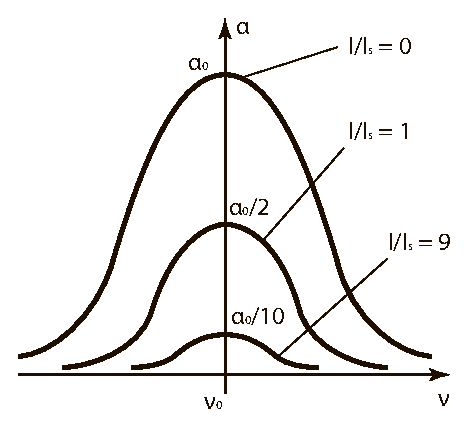
\includegraphics[width=.4\textwidth]{07_03}
\end{figure}

Вывод: при увеличении интенсивность насыщающего излучения коэффициент
поглощения уменьшается, а форма линий остаётся такой же, определяемая
однородным усилением.

\subquestion{Коэффициент усиления активной среды}

В поглощающей среде \( n_1 > n_2 \Rightarrow \alpha = \sigma(n_1 - n_2) > 0 \).

В усиливающей среде \( n_1 < n_2 \Rightarrow K = \sigma(n_2 - n_1) > 0 \),
где \( K \)~-- коэффициент усиления.
\[
    K = \sigma(n_2 - n_1); \quad K = \frac{K_0}{1 + I / I_s},
\]
где \( K_0 \)~-- коэффициент усиления при \( I = 0 \).

\begin{figure}[h]
    \center
    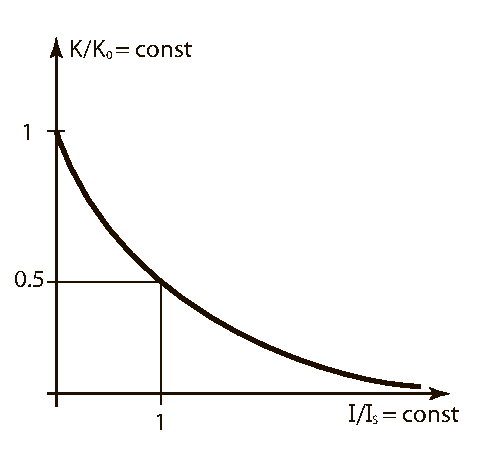
\includegraphics[width=.4\textwidth]{07_04}
\end{figure}

По мере роста интенсивности усиливающего излучения коэффициент излучения падет
и стремится к нулю.
